\documentclass[10pt,a4paper]{article}
\usepackage[T1]{fontenc}
\usepackage[utf8]{inputenc}
\usepackage{mathptmx}
\usepackage[margin=21mm,headheight=14pt]{geometry}
\usepackage{microtype,graphicx,booktabs,tabularx,array,amsmath,amssymb}
\usepackage[table]{xcolor}
\usepackage{caption,placeins,fancyhdr,enumitem}
\usepackage[numbers,sort&compress]{natbib}
\usepackage{hyperref}
\definecolor{ink}{HTML}{173541}
\definecolor{teal}{HTML}{087F8C}
\definecolor{wash}{HTML}{EDF5F5}
\hypersetup{colorlinks=true,linkcolor=teal,citecolor=teal,urlcolor=teal,
 pdftitle={Collaborative LiDAR Mapping with Multi-Layer BEVs and Belief Sharing on Robot-Decoupled Submap Graphs},
 pdfauthor={Research technical report}}
\captionsetup{font=small,labelfont=bf,labelsep=period}
\captionsetup[table]{position=top,skip=6pt}
\setlength{\parskip}{3pt}
\setlength{\parindent}{1em}
\setlength{\textfloatsep}{13pt}
\setlength{\intextsep}{12pt}
\renewcommand{\arraystretch}{1.14}
\setlist[itemize]{nosep,leftmargin=1.4em}
\pagestyle{fancy}\fancyhf{}
\fancyhead[L]{\small\color{ink}Multi-layer BEVs and belief sharing on submap graphs}
\fancyhead[R]{\small Technical report / 2026-10-05}
\fancyfoot[C]{\small\thepage}
\renewcommand{\headrulewidth}{.3pt}
\newcommand{\SE}{\mathrm{SE}}
\newcommand{\R}{\mathbb{R}}
\newcommand{\ate}{\operatorname{ATE}}
\begin{document}
\thispagestyle{empty}
\begin{center}
{\small\scshape\color{teal}Technical report\quad /\quad 5 October 2026}\par\vspace{7pt}
{\LARGE\bfseries\color{ink}Collaborative LiDAR Mapping with Multi-Layer BEVs\par
and Belief Sharing on Robot-Decoupled Submap Graphs}\par\vspace{7pt}
{\normalsize Multilayer place recognition, fixed spatial footprints, and persistent distributed optimization}
\end{center}
\vspace{-3pt}
\begin{abstract}
Collaborative LiDAR mapping must recover a common frame from observations with different viewpoints while controlling submap redundancy and distributed optimization cost. We describe a pipeline combining persistent-map EllipseLIO odometry, incrementally placed fixed-radius circles, gravity-aligned point-cloud bird's-eye views, terrain-relative multilayer matching, geometric verification, pairwise consistency maximization, and persistent Contractive Belief Sharing with GPU registration factors. Circle locations remain fixed while their geometry accumulates before immutable publication. In a simultaneous $1\times$ replay of all eight aerial and six ground GRACO sequences, the pipeline forms one 14-robot component during playback. The final settled result contains 366 submaps and 111 retained loops, achieves 0.933\,m joint position ATE, and exchanges 546.77\,MB of serialized inter-robot application payload. The largest component contains only four robots in an ablation that freezes geometry immediately. Across 842 measured nonterminal updates, median solver and full timer-callback times are 0.351 and 1.629\,ms, respectively; no sharp update-cost increase appears at the observed local graph sizes. These results establish operation at the tested scale on one workstation, with explicit limits on timing coverage, comparison scope, and extrapolation to physical networks or embedded hardware.
\end{abstract}
\begin{figure}[h!]
\centering
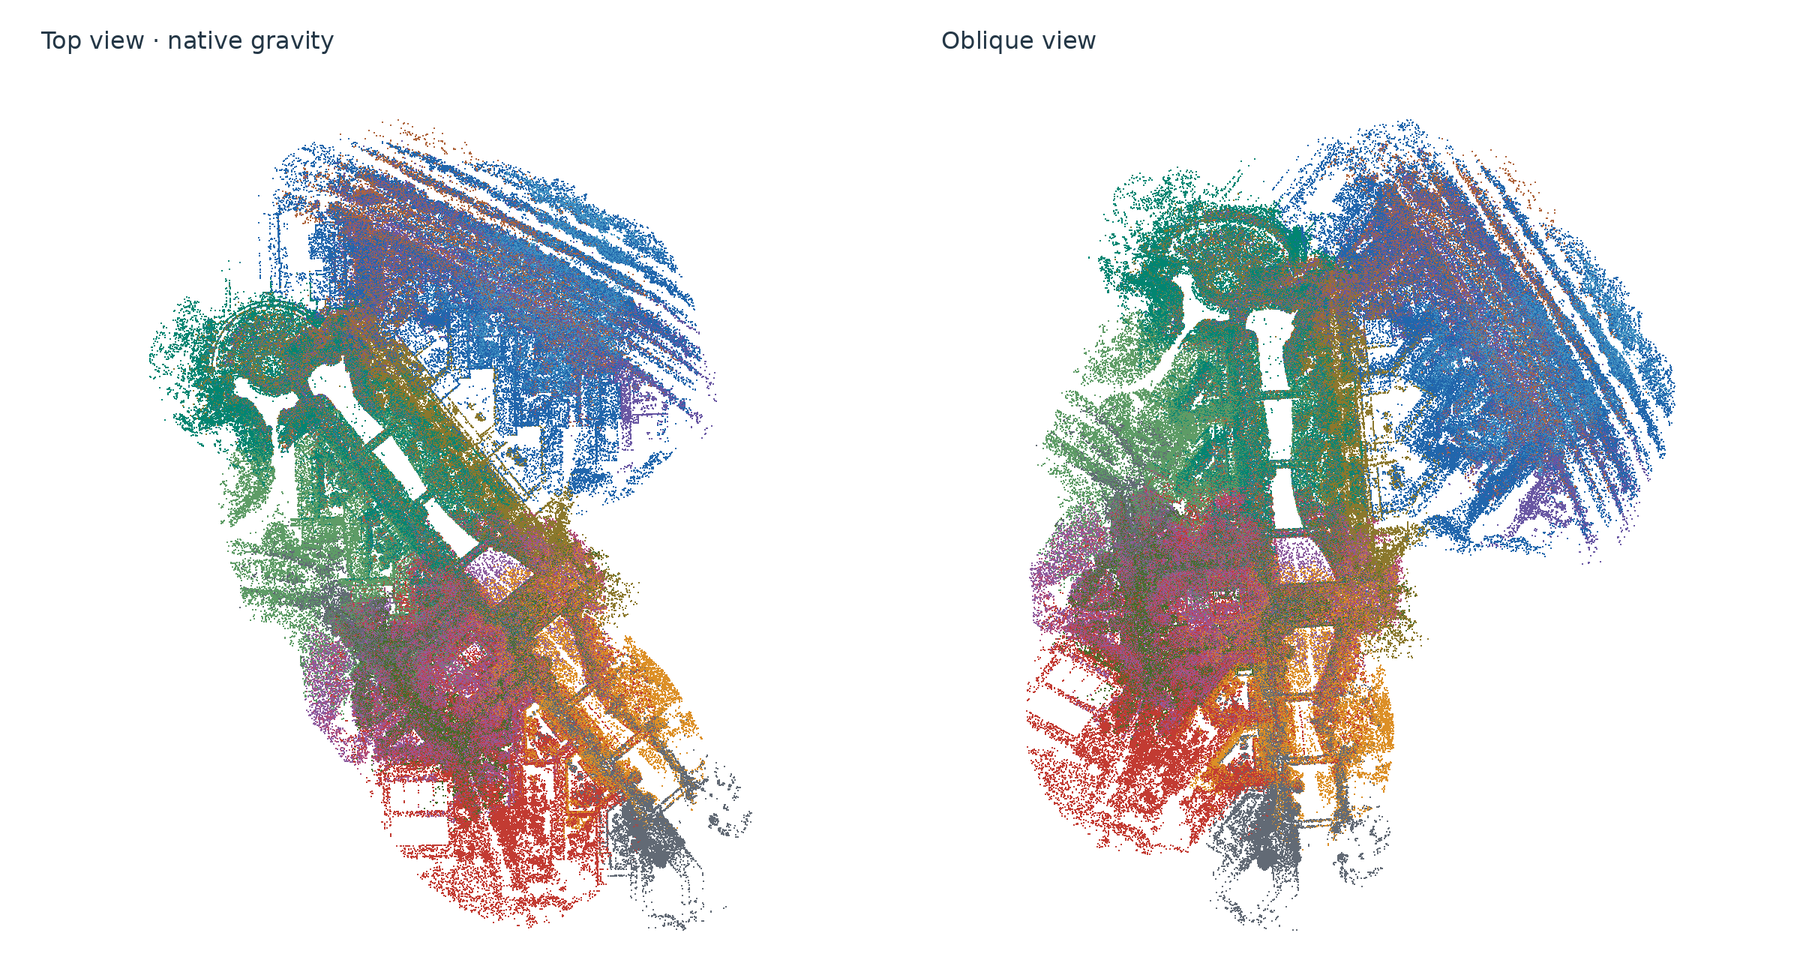
\includegraphics[width=\linewidth]{../figures/online-global-map.png}
\caption{The current pipeline's final joint map from all 14 GRACO sequences, viewed from above and obliquely. Robot colors distinguish contributions. The PLY contains 13.35 million unique retained native map representatives, re-posed by optimized submaps; the preview is thinned for display. A single native-gravity rotation sets the viewing frame. Ground truth is not used for map assembly.}
\label{fig:joint-map}
\end{figure}
\clearpage
\section{Problem and system design}
\label{sec:method}
A collaborative map requires accurate relative placement of robots, beyond accurate independently aligned trajectories. Ground and aerial robots may revisit the same place while observing different surfaces or height ranges. Submaps must therefore contain enough shared spatial structure for retrieval and verification, while remaining economical to exchange and optimize. Our design separates three decisions: where a submap lies, when its geometry is ready to publish, and how its pose is refined in the shared graph.

Each robot runs EllipseLIO~\cite{ellipselio} against its persistent local map. The collaborative backend consumes native retained point representatives, forms spatial submaps, retrieves potential overlaps using MapClosures~\cite{mapclosures}, verifies them with point-cloud registration, and optimizes the resulting submap graph using distributed CBS~\cite{cbs}. Odometry state, covariance, calibration and IMU propagation remain continuous. Circle handovers do not change the odometry map. The backend representation described here is point-cloud based; the ellipsoid representation belongs to the odometry frontend.

\subsection{Incremental placement independent of the trajectory}
Each robot places circles in one fixed gravity-horizontal frame using observed map geometry. The current capture interface supplies chronological 80\,m native area observations, triggered by 20\,m horizontal travel or 10\,s. Their growing union contains unique native point IDs available so far. It is not a complete archive of all raw scans. Robot poses provide coordinate transformations and creation anchors, but are not candidate inputs to the circle-position optimizer.

Let $\mathcal{U}_r(t)$ be that union for robot $r$, and $\Pi_r$ its fixed horizontal projection. Occupied 1\,m grid cells, with fixed origin, are counted once regardless of point density or observation height. Let $\mathcal{G}_r(t)$ denote their centers. A circle has fixed radius $R=40$\,m and center $c_{rk}\in\R^2$. The coverage constraint is
\begin{equation}
 \frac{1}{|\mathcal{G}_r(t)|}\sum_{g\in\mathcal{G}_r(t)}
 \mathbf{1}\!\left[\min_k\|g-c_{rk}\|\le R\right]\ge0.99.
 \label{eq:coverage}
\end{equation}
Existing centers and IDs remain immutable. When new observations lower coverage below the target, deterministic farthest-point selection generates candidate centers from uncovered cells until each is within $R/4$ of a candidate. A sparse candidate-to-cell coverage matrix supports a greedy feasible cover followed by a HiGHS mixed-integer solve minimizing the number of new circles. The solve has a 10\,s time limit and retains the greedy solution if no validated feasible incumbent is available.

Only new centers may be refined continuously. Refinement reduces deviation of each circle's greatest neighbor overlap from a 30\% target while protecting enough covered cells to preserve Eq.~\eqref{eq:coverage}. Disk overlap is intersection area divided by $\pi R^2$; 20--40\% is the desired band, not a hard guarantee. Redundant new circles are removed only after exact coverage validation. Coverage takes priority over circle count, which takes priority over overlap. Any optimality certificate applies to the current candidate set, not to an unknown future map or a globally minimal lifelong cover.

\subsection{Maturing geometry in a fixed footprint}
Footprint coverage does not ensure that the geometry currently inside a circle is useful for place recognition. We therefore create each footprint immediately but postpone its publication. While it is pending, it accumulates every newly available native representative inside that fixed circle, regardless of scan membership. There is no additional vertical crop or scan-age cutoff.

Normal publication requires at least 30\,s of sensor-time age, at most 5\% growth in both unique point IDs and occupied cells over a trailing interval of at least 30\,s, a supported terrain fit, and at least five ORB features summed across the height bands. Circles publish in permanent ID order. A 120\,s sensor-time deadline bounds head-of-line waiting, checked at the next available observation. End-of-stream tails are also released. Deadline and tail releases retain their actual support status; they are not relabeled stable. This minimum-age policy does not promise 30\,s publication latency.

At sealing time $t_s$, the published support is
\begin{equation}
 \mathcal{S}_{rk}=\{p\in\mathcal{U}_r(t_s):\|\Pi_r(p)-c_{rk}\|\le R\}.
\end{equation}
Geometry is expressed in the IMU frame of the original creation scan. The circle center, creation pose and pose timestamp never move to the latest robot position. Separate creation, seal and wall-availability timestamps prevent peers from querying future geometry. Payload hashes bind the descriptor, registration evidence and endpoint metadata. After publication, geometry is immutable; later observations remain available to pending circles and final map visualization but do not silently revise existing factors.

\subsection{Point-cloud BEVs and multilayer matching}
Sealed point clouds are projected onto gravity-horizontal density images at 0.5\,m resolution, using the pinned MapClosures normalization, density threshold 0.05, ORB extractor, Hamming threshold 50 and HBST retrieval. The exchanged representation comprises local ORB descriptors and metric feature coordinates, rather than one global descriptor vector per submap. Candidate similarity supplies a geometric hypothesis, not a guarantee of three-dimensional overlap.

Terrain-relative bands address the height-dependent structures visible to ground and aerial platforms. A spatially balanced low-surface estimator uses the 10th-percentile height of supported 4\,m cells, with at least 20 points per cell. Its plane fit uses 600 seeded hypotheses, 0.35\,m tolerance, at most $12^\circ$ slope, at least 30 supported cells, at least 15\% support, and 8\,m minor-axis spread. Relative height above this plane defines five bands: $[-0.5,2)$, $[2,5)$, $[5,10)$, $[10,20)$ and $[20,\infty)$ metres. This geometric layering is motivated by multi-BEV place recognition~\cite{forestlpr}; it does not use a learned global descriptor. A supported low surface need not be semantic ground. A failed terrain fit disables the layered query; full-height inspection images are not a retrieval fallback in this configuration.

Same-band ORB matches are merged in metric horizontal coordinates, with duplicate endpoint pairs consolidated before joint planar RANSAC. The estimator uses 688 seeded layer-balanced trials, 1.5\,m residual tolerance, one-to-one support within 0.5\,m, and more than five inliers. At most 20 candidate hypotheses are ranked per query; the live verifier admits at most two per query under its queue budget. Same-robot temporal exclusion is 30\,s. These are implementation settings, not accuracy guarantees implied by the referenced methods.

\subsection{Geometric verification and graph factors}
The planar seed is lifted through the gravity transforms, then initialized vertically from the point geometry. The initializer uses 0.8\,m voxels, horizontal neighbors within 1\,m, 0.5\,m height-vote bins and at most five separated modes. It does not use the robot's known flight height or ground truth. Point-cloud GICP~\cite{gicp,smallgicp} refines and verifies the seed using 0.4\,m evidence voxels, a 1.5\,m correspondence radius, 0.6\,m inlier radius, at least 100 inliers, at least 30\% overlap, and at most 0.35\,m inlier RMSE, with observability and conditioning checks.

Verified loops undergo PCM at probability 0.99 with minimum clique size one. A singleton loop may therefore be retained without a second loop corroborating it. Only PCM-retained loops can admit live GPU VGICP factors. The registration adapter uses the native \texttt{gtsam\_points} kernel family, up to 12,000 points per endpoint, 0.5\,m preprocessing, 20 covariance neighbors, and two adaptive voxel levels. The recorded factor maps use 1 and 2\,m voxel resolutions. Initial support checks can reject a geometry factor while preserving its companion verified pose constraint. A conservative information-ratio cap of one limits the registration contribution. Pose and geometry factors reuse observations and are not independent measurements.

\subsection{Persistent distributed optimization and reconstruction}
Each graph variable represents a fixed circle's creation-anchor pose; its ID follows the usual robot/submap endpoint contract. Local odometry supplies relations between creation anchors. Relative-pose loops and admitted geometry factors supply cross-submap constraints. Robot-local CBS optimizers, geometry caches and belief state persist while causal graph prefixes are admitted. Immutable endpoint/session validation and peer exchanges enforce ownership; no centralized optimization is used for the reported solution.

Each robot requests an update every 10\,s. Outgoing pose or anchor exchange is selected randomly each iteration, not in a strict alternating schedule. Both categories update the local graph; they are not separate solver kernels. Anchor beliefs propagate through the connected component, and a common-reference check precedes the final 30 settling iterations. A requested update period is distinct from complete graph-admission, shared-frame publication or convergence latency.

For raw and optimized creation poses $\widehat{X}_{rk}$ and $X_{rk}$, define correction $C_{rk}=X_{rk}\widehat{X}_{rk}^{-1}$. Dense trajectory reconstruction averages corrections sharing one creation timestamp, using mean translation and mean rotation, then interpolates translation and rotation (SLERP) between consecutive timestamps. It applies the resulting correction to every native odometry pose. Map reconstruction instead uses each circle's actual optimized correction: each retained point is assigned to its nearest footprint center and emitted once per robot-local native ID. Points outside all footprints are retained with the nearest correction and flagged. Neither reconstruction introduces a new registration or ground-truth alignment.

\section{Experimental protocol}
\label{sec:protocol}
The experiment assigns one logical robot to each of GRACO's~\cite{graco} eight aerial and six ground sequences. All 14 converted sensor streams replay simultaneously at $1\times$ on workstation 148. Each robot runs fresh calibrated EllipseLIO, circle preparation, point-cloud BEV retrieval and verification, and persistent distributed PCM/CBS during playback. Peers exchange actual DDS messages with isolated geometry ownership. The result is a simultaneous online replay on one workstation, not a physical 14-radio deployment or an embedded-hardware benchmark.

Native frontends use dataset- and robot-specific calibration, reliable sensor input, four ROS callback threads, and one numerical-library thread per process. No CPU, memory or GPU quotas are imposed. The effective native configurations and per-robot CBS YAML files, rather than unused inherited profile fields, define the run. Odometry validation requires complete finite chronological output, speed below 20\,m/s, and no post-initialization gap of at least 1\,s between successful LiDAR updates. Ground truth is confined to post-run evaluation.

Position accuracy uses evo~1.36.5 with 50\,ms association, rigid $\SE(3)$ alignment and no scale fitting. GRACO reference positions are expressed at the IMU; the separate ground/aerial calibrations are used consistently. For matched sets $\mathcal{I}_r$, joint ATE is
\begin{equation}
 \ate_{\mathcal{C}}=\sqrt{\frac{\sum_{r\in\mathcal{C}}\sum_{i\in\mathcal{I}_r}
 \|R_{\mathcal{C}}\widehat p_{ri}+t_{\mathcal{C}}-p^{\mathrm{GT}}_{ri}\|^2}
 {\sum_{r\in\mathcal{C}}|\mathcal{I}_r|}}.
\end{equation}
One shared transform is fitted for the whole confirmed component. This pose-weighted RMSE differs from averaging independently aligned robot errors. A disconnected team has no valid all-team joint ATE. Map assembly uses optimized poses and native gravity only.

\section{Fourteen-robot online results}
\label{sec:results}
All 14 robots form one shared component at 430.46\,s after playback release, before the last bag ends at 520.05\,s. The final publication is at 909.19\,s, including 389.14\,s after the last bag; total measured process lifetime is 913.15\,s. The final accuracy therefore describes the settled output of an online run, not accuracy at the instant playback ends. Thirteen growing graph revisions are admitted and each robot completes 60--62 persistent iterations, including final settling.

The final graph contains 366 submaps and 111 retained loops. Of 120 candidates reaching three-dimensional verification, 111 are accepted and all 111 survive PCM. Of those loops, 110 admit GPU registration factors and pass final support checks. The G02/26--G04/4 pair has initial overlap 0.289, below the unchanged 0.30 geometry-factor gate; only its companion pose constraint remains. Zero PCM rejection in this run does not establish zero false positives, and overlapping evidence makes loop counts dependent.

The all-14 joint ATE is 0.933\,m over 45,397 associated poses. Table~\ref{tab:robot-accuracy} distinguishes independently aligned trajectory shape from placement under the shared transform. CBS need not improve every robot's independent ATE while establishing a shared map. All odometry streams pass validation: maximum recorded speed is 5.43\,m/s and the largest successful-update gap is 0.472\,s.
\begin{table}[htbp]
\centering\small
\caption{GRACO position ATE (RMSE, metres). Raw and CBS individual columns each fit a separate rigid transform per robot. The shared column applies one transform to the entire connected team.}
\label{tab:robot-accuracy}
\begin{tabular}{lrrrrr}
\toprule
Robot & Circles & Matched poses & Raw, individual & CBS, individual & CBS, shared \\
\midrule
A01 & 31 & 3,832 & 0.180 & 0.300 & 0.721 \\
A02 & 15 & 2,572 & 0.061 & 0.061 & 0.283 \\
A03 & 22 & 3,685 & 0.065 & 0.224 & 0.675 \\
A04 & 22 & 2,747 & 0.115 & 0.115 & 0.318 \\
A05 & 30 & 2,763 & 0.173 & 0.204 & 1.164 \\
A06 & 19 & 3,107 & 0.064 & 0.065 & 0.758 \\
A07 & 24 & 3,714 & 0.075 & 0.074 & 0.457 \\
A08 & 21 & 2,617 & 0.123 & 0.245 & 0.517 \\
G01 & 23 & 3,102 & 0.297 & 0.292 & 1.035 \\
G02 & 30 & 3,634 & 0.649 & 0.679 & 1.601 \\
G03 & 24 & 2,780 & 0.598 & 0.584 & 1.184 \\
G04 & 30 & 3,075 & 0.515 & 0.494 & 0.996 \\
G05 & 46 & 4,877 & 0.477 & 0.462 & 0.764 \\
G06 & 29 & 2,892 & 0.443 & 0.446 & 1.429 \\
\textbf{All 14} & 366 & 45,397 & --- & --- & \textbf{0.933} \\
\bottomrule
\end{tabular}
\par\vspace{5pt}\begin{minipage}{0.97\linewidth}\footnotesize A01--A08 are aerial; G01--G06 are ground. The all-14 entry is pose-weighted joint RMSE, not the mean of row RMSEs. Independent alignment can hide relative placement error.\end{minipage}
\end{table}


The exported map contains 13,353,004 unique native representatives (Fig.~\ref{fig:joint-map}). Its gravity-aligned PLY retains robot colors, submap ownership and an uncovered-point flag, without an additional export voxel filter. The 31,212 representatives outside every footprint receive the nearest correction and remain visible. Independent PLY readback, per-robot counts and finite coordinates pass validation; a visual map is not itself an accuracy measurement.

\subsection{Ablation: the geometry-publication policy}
\label{sec:ablation}
Immediate geometry freezing tests whether geometric footprint coverage alone supplies adequate retrieval support. The ablation uses the same circle settings, odometry calibration, terrain estimator, matching and verification thresholds, PCM, and GPU registration settings. Its independent fresh replay is not an exactly frozen-input experiment; small differences in odometry and circle count remain. One execution per setting provides descriptive evidence, without repeated-trial confidence intervals.
\begin{table}[htbp]
\centering\small
\caption{Geometry-publication ablation on simultaneous all-14 replays. All placement, retrieval and verification thresholds are retained. Each column is a separate fresh execution.}
\label{tab:maturation-ablation}
\begin{tabular}{lrr}
\toprule
Measure & Immediate freezing & Maturation (current) \\
\midrule
Circle nodes & 358 & 366 \\
Connected components & 11 & 1 \\
Largest component (robots) & 4 & 14 \\
Retained loops & 4 & 111 \\
Empty layered descriptors & 197 & 74 \\
Final observed IDs in published evidence & 34.7\% & 91.5\% \\
All-team joint ATE (m) & Unavailable & 0.933 \\
Application traffic (MB) & 128.32 & 546.77 \\
\bottomrule
\end{tabular}
\par\vspace{5pt}\begin{minipage}{0.97\linewidth}\footnotesize The disconnected immediate-freeze run has no all-team joint ATE. Native-ID evidence coverage is different from occupied-cell footprint coverage. Independent odometry and scheduling introduce small differences in circle placement; this is not a frozen-input or repeated-trial estimate.\end{minipage}
\end{table}


The largest recovered component increases from four to 14 robots when geometry matures before publication, while empty layered descriptors decrease from 197 to 74. Published evidence contains 91.5\% of final observed native point IDs, compared with 34.7\% under immediate freezing. These evidence fractions differ from the 99\% occupied-cell footprint target. Every nonempty completed placement update satisfies that target, with a measured minimum of 99.0003\%.

The current run publishes 188 circles after normal stability/support checks, 129 at their deadline, and 49 at end of stream. Median sensor-time age at publication is 110.47\,s; the maximum is 129.60\,s because deadlines are checked at observations. Thus support improves at the cost of delayed availability and greater traffic. The remaining 74 terrain failures have no layered features. This ablation supports maturation for the tested sequence, not a universal waiting policy or guaranteed semantic terrain identification.
\FloatBarrier

\section{Communication cost}
\label{sec:communication}
The current run exchanges 546.77\,MB of serialized remote application payload, or 39.05\,MB per assigned robot (Table~\ref{tab:traffic}). Counters include recipient fan-out, retrieval, verification geometry, retained constraints, PCM, registration exchange, and CBS requests and replies. CBS messages are counted once at the requester; PCM and geometry count sent payloads. Local sensor/visualization traffic, report downloads, middleware discovery, transport framing and retransmissions are excluded. These measurements characterize application traffic, not physical network bytes or delivered wireless throughput.
\begin{table}[htbp]
\centering\small
\caption{Measured remote application payload for the current GRACO all-14 run. One MB is $10^6$ bytes.}
\label{tab:traffic}
\begin{tabular}{lrr}
\toprule
Exchange & MB & Share (\%) \\
\midrule
Retrieval queries & 410.444 & 75.07 \\
Verification geometry replies & 110.565 & 20.22 \\
Candidate replies & 2.916 & 0.53 \\
Verified constraints & 0.350 & 0.06 \\
Geometry requests & 0.109 & 0.02 \\
Peer completion messages & 0.014 & 0.00 \\
PCM exchange & 1.206 & 0.22 \\
CBS registration geometry & 17.752 & 3.25 \\
CBS belief requests and replies & 3.412 & 0.62 \\
\textbf{Total} & \textbf{546.767} & \textbf{100.00} \\
\bottomrule
\end{tabular}
\par\vspace{5pt}\begin{minipage}{0.97\linewidth}\footnotesize Recipient fan-out is counted. Middleware/transport headers, discovery and retransmissions are excluded; these are not physical link-byte measurements.\end{minipage}
\end{table}


Retrieval queries account for 410.44\,MB, or 75.1\% of total traffic. Requested verification geometry contributes 110.56\,MB. CBS belief traffic is 3.41\,MB, approximately 0.62\% of the total; it cannot stand in for whole-pipeline communication. Retrieval exchange is therefore the largest measured target for communication reduction, subject to maintaining detection and connectivity.

\begin{table}[htbp]
\centering\small
\caption{Communication context from completed native-baseline GRACO ground-trio runs and the current 14-robot mixed run. The workloads are different; per-robot normalization is descriptive.}
\label{tab:baseline-traffic}
\begin{tabular}{llrrr}
\toprule
Method & Assigned team & Connected & Total MB & MB/robot \\
\midrule
Swarm-SLAM~\cite{swarm} & G01--G03 & 3/3 & 96.12 & 32.04 \\
DCL-SLAM~\cite{dcl} & G01--G03 & 3/3 & 393.52 & 131.17 \\
DiSCo-SLAM~\cite{disco} & G01--G03 & 3/3 & 802.58 & 267.53 \\
\textbf{Current pipeline} & A01--A08, G01--G06 & 14/14 & 546.77 & 39.05 \\
\bottomrule
\end{tabular}
\par\vspace{5pt}\begin{minipage}{0.97\linewidth}\footnotesize All rows use serialized inter-robot application payload accounting. Different team size, trajectory length, observations and constraints preclude a matched efficiency or accuracy ranking. No incomplete measurement is included.\end{minipage}
\end{table}

The separate completed ground-trio measurements provide context for magnitude, rather than a same-workload ranking. All entries in Table~\ref{tab:baseline-traffic} connect their assigned team. Our per-robot total is approximately 3.4 times lower than DCL-SLAM's and 6.9 times lower than DiSCo-SLAM's, but 22\% higher than Swarm-SLAM's. Different team sizes, spatial support, trajectory durations and recovered constraints remain confounds; division by robot count does not remove them. The evidence supports a competitive measured communication cost, not an unconditional efficiency win over every baseline.
\FloatBarrier

\section{Computation as the graph grows}
\label{sec:computation}
Native timing logs separate the local solver update, the complete nonterminal timer callback, and peer-belief service responses. The analysis joins timing and statistics by robot and iteration, validates new-factor/value counts, and checks cumulative owned nodes against admitted graph prefixes. It retains 842 timed updates and 3,930 service requests. One terminal timer callback per robot is not recorded by the native CSV and is never filled with zero.
\begin{table}[htbp]
\centering\small
\caption{Native elapsed wall-time measurements. All duration columns are in milliseconds.}
\label{tab:timing}
\begin{tabular}{lrrrr}
\toprule
Timed region & Samples & Median (ms) & P95 (ms) & Maximum (ms) \\
\midrule
Local solver update & 842 & 0.351 & 1.003 & 4.499 \\
Full nonterminal callback & 842 & 1.629 & 32.230 & 1188.685 \\
Peer-belief service & 3,930 & 0.379 & 2.385 & 190.248 \\
\bottomrule
\end{tabular}
\par\vspace{5pt}\begin{minipage}{0.97\linewidth}\footnotesize The full callback contains the local solver update, so rows must not be added. Peer services run separately. Fourteen terminal callbacks, final geometry validation and pre-update early returns are outside the timing coverage.\end{minipage}
\end{table}


The solver call takes 0.351\,ms median and 4.499\,ms maximum. Its timer excludes input and geometry preparation. The broader callback takes 1.629\,ms median, 32.230\,ms at the 95th percentile, and 1.189\,s maximum, including the startup/admission spikes in Fig.~\ref{fig:timing-progress}. It includes lock waiting, successful input preparation, registration preparation, solver update, residual/statistics computation and asynchronous request submission. Calls returning before an update, separate PCM/geometry-exchange callbacks, and Python bridge work are outside this timer.

Peer-service timings separately include lock waiting, cavity marginalization and response packing. Their median is 0.379\,ms and maximum is 190.248\,ms. Services do not carry wall timestamps: plotting assigns each to its serving robot's iteration timestamp, with approximate temporal location. Five requests preceding iteration one appear only in the retained data and duration summary. Update plot timestamps are the corresponding statistics-receipt times. All durations are elapsed wall time from native timers, not CPU time or synchronized GPU kernel measurements.

\begin{figure}[p]
\centering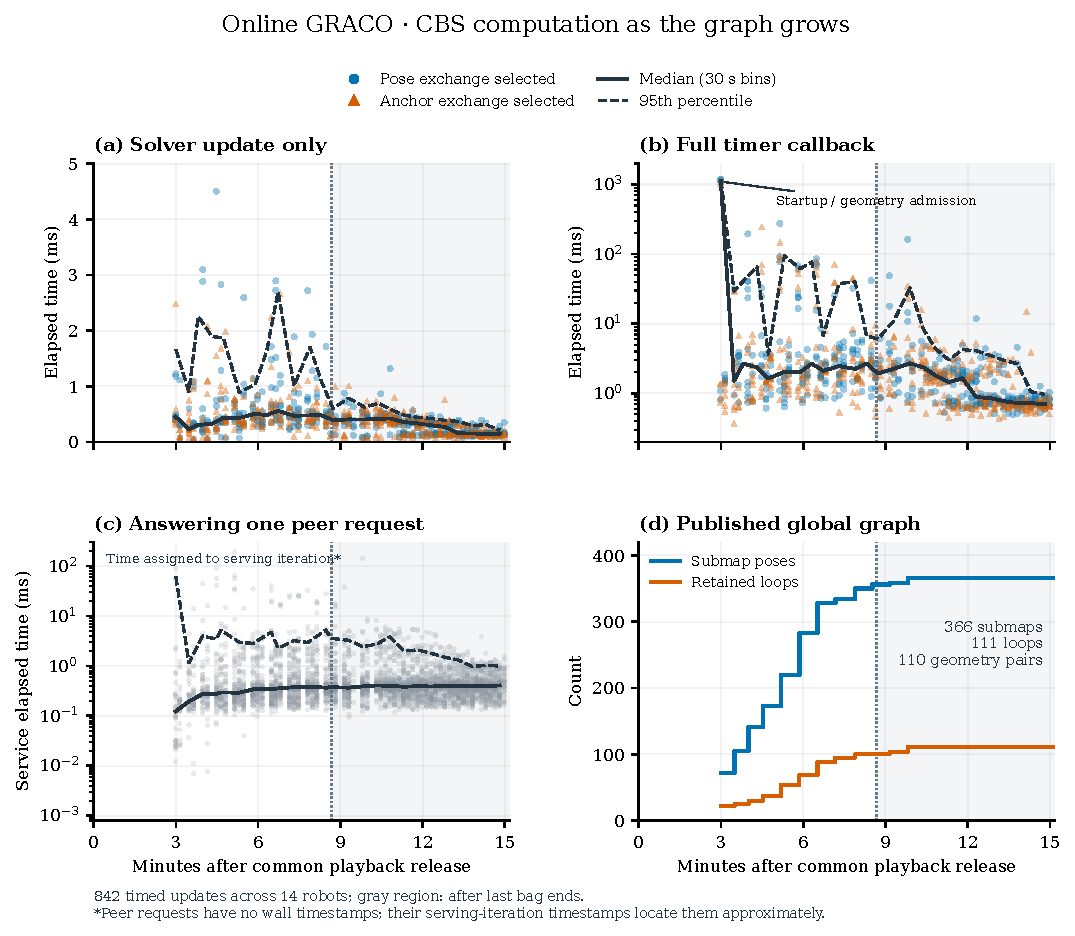
\includegraphics[width=\linewidth]{../output/pdf/cbs-update-progress.pdf}
\caption{CBS computation throughout the online experiment. Points are recorded local updates or service responses; solid and dashed curves show median and 95th percentile within 30\,s bins. Pose/anchor colors identify the randomly selected outgoing exchange after an update, not two separate solver kernels. The gray region follows the last bag's end. The graph grows to 366 submap poses and 111 retained loops, including 110 geometry pairs. Peer-service times are positioned approximately by serving iteration. No missing terminal timer values are imputed.}
\label{fig:timing-progress}
\end{figure}

The global graph is distributed across 14 optimizers: the largest recorded local estimate has 61 variables, including owned submaps, peer separator poses and anchors. Figure~\ref{fig:local-scaling} therefore relates cost to local variable count as well as global progress. No sharp update-cost increase appears within this tested range. The late reduction in cost coincides with fewer new factors and beliefs and a fixed graph; it does not show that larger graphs are intrinsically cheaper. One concurrent run with caching and varying geometry cannot establish an asymptotic complexity bound.

\begin{figure}[htbp]
\centering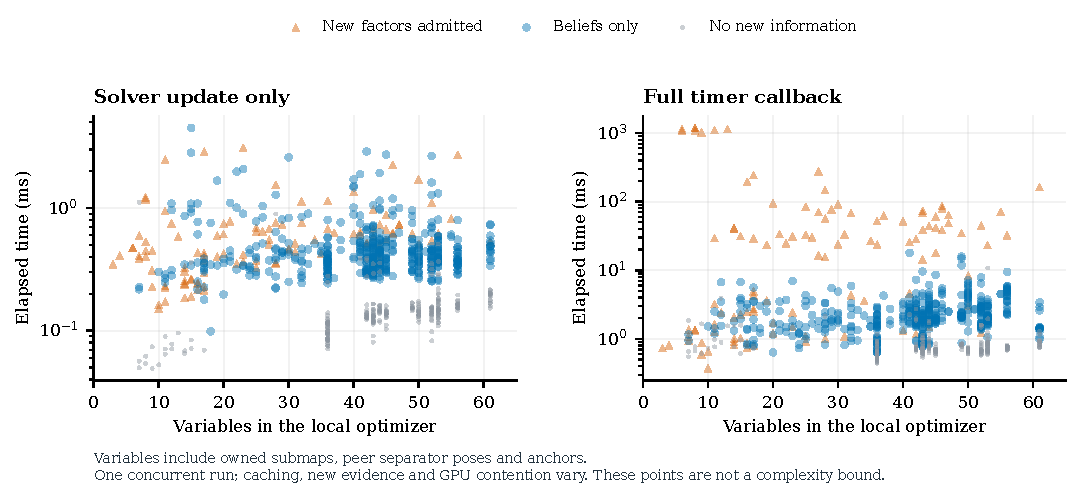
\includegraphics[width=\linewidth]{../output/pdf/cbs-local-graph-scaling.pdf}
\caption{Measured local computation versus optimizer variable count. New-factor admission has a distinct preparation cost, visible in full callbacks. Belief-only and no-new-information updates remain inexpensive over the observed range. Counts are local, not the global 366-node graph size; geometry budgets, graph structure and concurrent GPU load are not held constant.}
\label{fig:local-scaling}
\end{figure}

Short local computation is distinct from complete online latency. Asynchronous peer responses, prefix readiness, common-reference propagation and the configured settling schedule can delay publication while individual updates are inexpensive. The 10\,s update request does not promise a settled result every 10\,s. Final geometry validation, executed on the unlogged terminal path, is outside the reported timer maxima.

The full simultaneous pipeline, including odometry, preparation, recording and distributed processing, takes 913.15\,s wall time and 6,617.64 process-tree CPU seconds. Peak simultaneous process-tree RSS is 42.34\,GiB; shared pages may be counted multiple times. Whole-device GPU allocation peaks at 4,135\,MiB and includes device/driver overhead and any unrelated activity. These are all-14 workstation measurements, not per-robot memory requirements or Jetson Orin NX validation.
\FloatBarrier

\section{Limitations and interpretation}
The experiment demonstrates one successful concurrent 14-stream replay, with explicit reference propagation, finite odometry, validated registration support and measured application traffic. A single replay on one workstation does not establish operation over a bandwidth-limited radio network, repeated-run robustness, or embedded real-time performance. The 0.933\,m joint ATE includes post-playback settling. The report does not substitute independent robot alignments for that shared-frame result.

Fixed footprints control placement density but do not solve every evidence-management problem. The growing union and the number of fixed circles can increase over long missions. Geometry maturation delays the first useful query, and its deadline/tail releases can remain unsupported. Once published, a circle does not absorb later observations into its retrieval or registration evidence. The overlap target is subordinate to coverage and circle count. Necessary future tests include longer runs, repeated fixed-team experiments, and measured retrieval/geometry load as map size grows beyond the 61-variable local graphs observed here.

The focused ablation supports the publication policy under the tested settings; it does not isolate all contributions of layering, vertical initialization, placement or registration factors. PCM singleton acceptance supplies no pairwise corroboration, and reused geometry makes companion pose and registration factors statistically dependent. Final support checks are engineering safeguards rather than a proof that every retained loop is correct. Ground truth is used only after estimation, and a visually coherent map is not a replacement for trajectory evaluation.

The method's accuracy evidence here is limited to the GRACO team and the specified maturation ablation. This report does not assign current-pipeline accuracy to untested datasets or use different baseline team sizes as a matched ranking. S3E and Jetson deployment require evaluation of this exact configuration before corresponding claims can be made.

\section{Conclusion}
Incrementally placed fixed circles separate spatial submap support from the robot trajectory, while geometry maturation supplies more complete evidence before immutable publication. With point-cloud multilayer retrieval, verified loops and persistent GPU-assisted CBS, the pipeline connects all 14 GRACO streams during playback and reaches 0.933\,m final joint ATE. Its 546.77\,MB measured application traffic is dominated by retrieval queries; local CBS calls remain inexpensive across the observed graph growth. The evidence supports the tested configuration and identifies publication latency, retrieval traffic and longer-horizon resource growth as the next evaluation priorities.

\FloatBarrier
\bibliographystyle{unsrtnat}
\bibliography{references}
\clearpage
\appendix
\section{Reproducibility and validation}
\label{sec:reproducibility}
The run identifier is \texttt{circle-mature-online148-20261001/full}. Immutable bulk captures and recordings remain on workstation 148. The report source package retains the current configuration, native configuration identities, source and binary hashes, accuracy results, communication counters, timing summaries, and publication audits. Tables are generated directly from these saved JSON records; report generation does not rerun SLAM, fit trajectories or change acceptance thresholds.

Post-run inspection identifies workstation 148 as an Intel Core Ultra 9 285K host with 24 visible logical CPUs, approximately 62.25\,GiB OS-visible RAM, and an NVIDIA GeForce RTX 5080 (16,303\,MiB reported device memory). The retained inventory is labeled post-run; it is not a record of experiment-time clock rates or utilization.

The effective settings are summarized in Table~\ref{tab:settings}. Native calibrated frontend files and per-robot CBS YAML take precedence over inherited unused configuration fields. In particular, execution is persistent with a 0.1\,Hz requested update rate and 30 final settling iterations. The point-cloud renderer and terrain-relative retrieval policy define the reported backend.
\begin{table}[htbp]
\centering\small
\caption{Effective configuration of the reported online run.}
\label{tab:settings}
\begin{tabular}{lp{0.68\linewidth}}
\toprule
Component & Setting \\
\midrule
Odometry & Persistent native EllipseLIO; calibrated IMU frame \\
Circle footprint & Radius 40\,m; 1\,m occupied-cell grid; 99\% coverage \\
Placement priorities & Coverage, circle count, then 30\% overlap target \\
Placement solve limit & 10\,s per update; validated greedy fallback \\
Normal geometry publication & Age $\geq$30\,s; growth $\leq$5\% over $\geq$30\,s; terrain/feature gates \\
Forced publication & 120\,s deadline at next observation, or end of stream \\
BEV retrieval & Point density, 0.5\,m pixels; five terrain-relative bands \\
Point-GICP verification & 0.4\,m evidence voxels; 1.5\,m correspondence radius \\
PCM & Probability 0.99; minimum clique size one \\
Registration factors & Native GPU VGICP; 0.5\,m preprocessing; 12,000 points/endpoint \\
Factor voxel levels & Two adaptive levels; recorded maps at 1 and 2\,m \\
Persistent CBS & 0.1\,Hz requested; random outgoing pose/anchor exchange \\
Final settling & Common-reference barrier, then 30 iterations \\
Evaluation & evo 1.36.5; 50\,ms association; shared rigid alignment; no scale \\
\bottomrule
\end{tabular}
\end{table}


An independent audit reconstructs every published payload from its seal-time observation prefix, checking member IDs, coordinates, creation anchors, hashes and descriptor/evidence agreement. Graph-prefix checks establish causal availability and both-endpoint receipt before loop admission. All final admitted registration factors pass support checks; published loop transforms satisfy the common-frame contract. The retained focused test run has 38 passes and three native-gated skips, supplemented by the actual distributed run checks. All 14 Rerun recordings pass footer-inclusive validation, and independent PLY readback confirms counts, finite coordinates and colors.

The numerical evidence used by the report is under \path{evidence/}. In particular, \path{audit.json} contains availability, odometry health and byte accounting; \path{evaluation.json} supplies the shared and individual trajectory errors; \path{cbs-timing/summary.json} supplies timing distributions and joins; and \path{baseline-communication.json} preserves the explicitly scoped comparator measurements. Source hashes and a machine-readable report check record are included. The compact source bundle can compile without dataset bags, bulk maps, remote access or a plotting runtime.

\begin{figure}[p]
\centering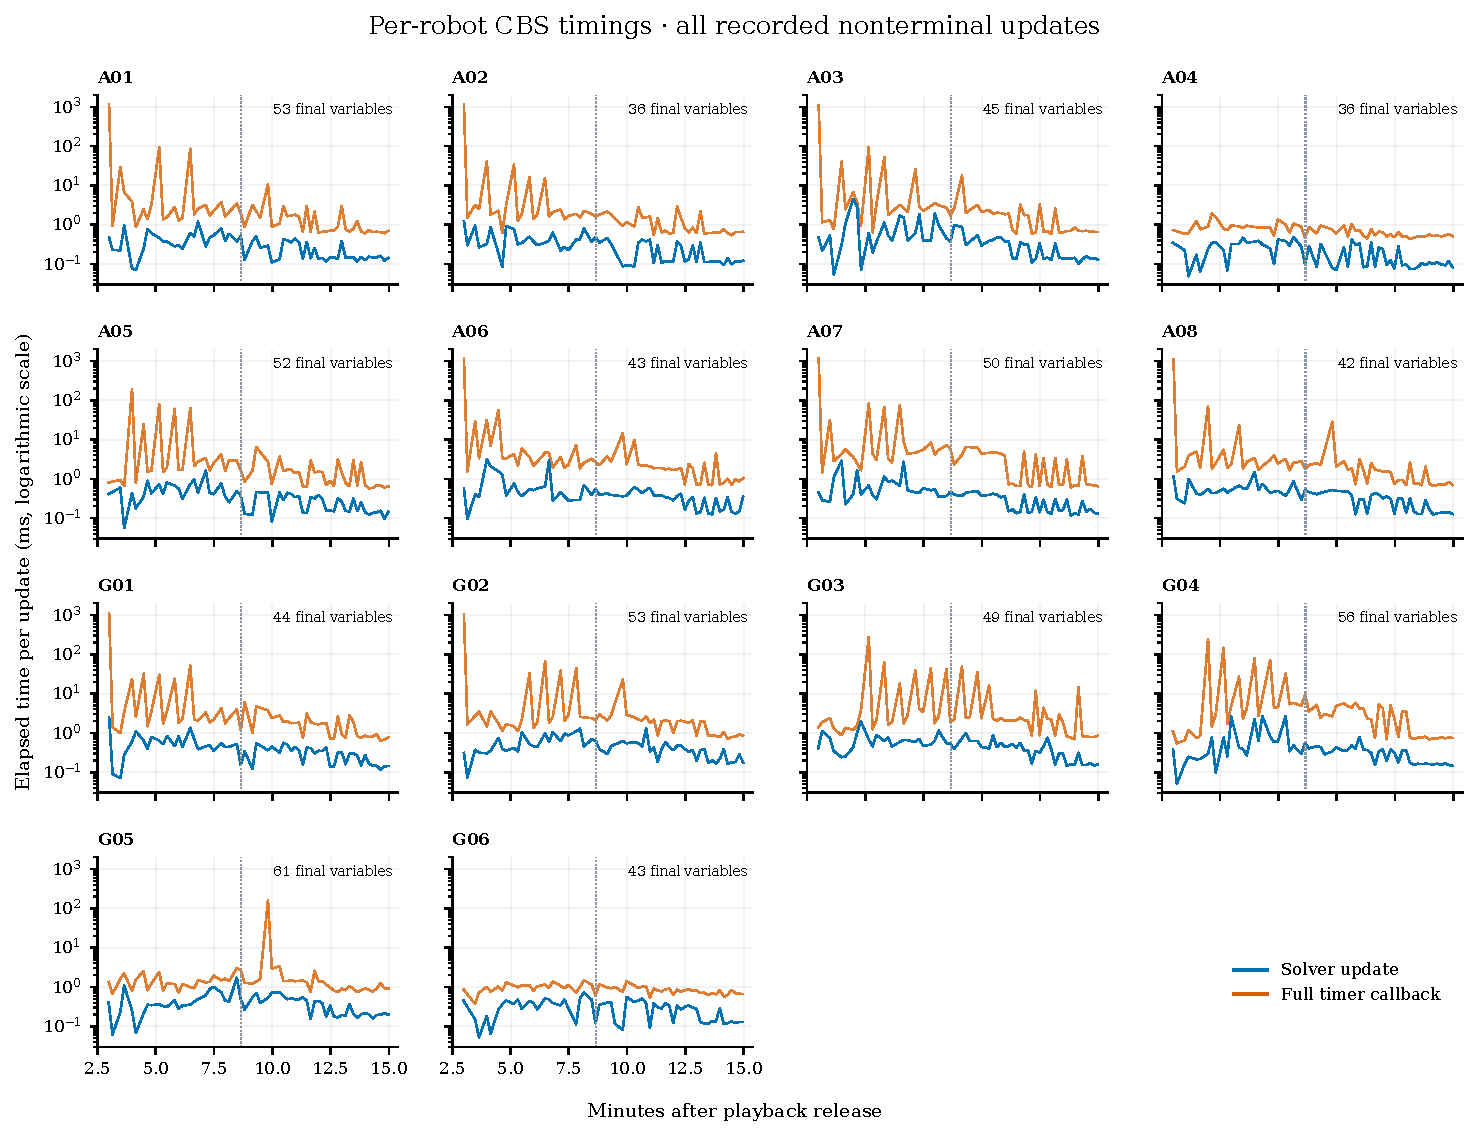
\includegraphics[width=\linewidth]{../output/pdf/cbs-per-robot-progress.pdf}
\caption{All 14 robots' nonterminal timing records. Blue is the solver update and orange the broader timer callback. Dotted lines mark the last bag's end. The logarithmic axis preserves admission spikes and low-cost updates in one view. Final variable counts include local and separator poses and anchors.}
\label{fig:per-robot}
\end{figure}
\FloatBarrier

\end{document}
